\documentclass[11pt,a4paper]{article}
\usepackage[T1]{fontenc}
\usepackage{lmodern}
\usepackage{amsmath,amssymb,amsthm,mathtools}
\usepackage[margin=25mm]{geometry}
\usepackage{microtype,booktabs,array,xcolor,tikz,hyperref}
\usetikzlibrary{arrows.meta,positioning,calc,fit,backgrounds}
\definecolor{ink}{HTML}{18334A}
\definecolor{blue}{HTML}{176B99}
\definecolor{teal}{HTML}{087F71}
\definecolor{rust}{HTML}{B74E32}
\definecolor{pale}{HTML}{EFF5F8}
\hypersetup{colorlinks=true,linkcolor=blue,citecolor=teal,urlcolor=blue}
\newtheorem{theorem}{Theorem}[section]
\newtheorem{lemma}[theorem]{Lemma}
\newtheorem{proposition}[theorem]{Proposition}
\theoremstyle{definition}
\newtheorem{definition}[theorem]{Definition}
\newcommand{\PT}{\operatorname{PT}}
\newcommand{\inv}{\operatorname{inv}}
\newcommand{\inc}{\operatorname{inc}}
\newcommand{\sh}{\operatorname{sh}}
\newcommand{\N}{\mathbb N}
\newcommand{\cell}[4]{\draw[draw=ink,fill=#4,rounded corners=1pt] (#1,#2) rectangle ++(.68,.68);\node[text=ink] at (#1+.34,#2+.34) {$#3$};}
\newcommand{\tagline}[1]{\par\smallskip\noindent\textcolor{teal}{\small\textsf{#1}}\par\smallskip}
\title{\textcolor{ink}{From a Failed Corner Slide\\to a Verified Tableau Injection}\\[3mm]
\large A constructive positivity proof in height two,\\with exact obstructions and Lean-checked survivor counts}
\author{Yamba AI Math Lab\\\small Research note prepared for Christopher Yamba}
\date{21 October 2026}

\begin{document}
\maketitle
\begin{abstract}
An earlier research conversation proposed a universal sign-reversing tableau
involution for elementary coefficients of chromatic quasisymmetric functions.
The proposed corner slide fails on five vertices, even for a connected
incomparability graph of a height-two poset. We give its exact validity
criterion and show an infinite cardinality obstruction to its intended
unrestricted shape-to-shape injection. Allowing the moved entry to pass an
initial block of comparable entries repairs validity; the absence of a
three-element chain makes this repair injective. This construction is the
existing injection of Cho--Huh, which we independently recovered and explicitly
attribute. We give a complete mathematical proof of the height-two positivity
corollary, reproducible finite calculations, and a precise account of which
combinatorial statements are checked by Lean. The certificate now includes
complete finite tableau families and a survivor-count identity in every
inversion degree, including all boundary indices. We do not claim a new proof of
general positivity, a novel injection, or a fully formalized symmetric-function
theorem.
\end{abstract}

\begin{center}
\fcolorbox{teal}{pale}{\parbox{.9\linewidth}{\small
\textbf{Claim status.} The original universal slide is \textbf{refuted}.
The local repair and height-two injection are \textbf{proved} below.
Height-two positivity is an \textbf{established result reproduced here}.
Finite computations are \textbf{empirical, exact, and bounded}.
The full research objective remains \textbf{unresolved in this project}.}}
\end{center}

\section{The problem and its actual frontier}

For a labeled graph $G$ on $[n]$, a proper coloring is a map
$\kappa:[n]\to\N_{>0}$ assigning distinct colors to adjacent vertices. Set
\[
 X_G(\mathbf x;q)=\sum_{\kappa\text{ proper}}
 q^{\operatorname{asc}_G(\kappa)}\prod_{i=1}^n x_{\kappa(i)},
 \quad
 \operatorname{asc}_G(\kappa)=\#\{ij\in E:i<j,\ \kappa(i)<\kappa(j)\}.
\]
For a natural unit interval graph this is symmetric. Its elementary expansion is
\[
 X_G=\sum_{\lambda\vdash n}c_\lambda(q)e_\lambda,
\]
where
$e_\lambda=\prod_i e_{\lambda_i}$.
The constructive goal is to interpret every $c_\lambda(q)$ as a sum of
nonnegative monomials, ideally through a uniform, explicitly invertible map.

\tagline{Established context; theorem statements inspected, not full proof audits}
Hikita proved ordinary Stanley--Stembridge positivity; his result gives
nonnegativity at positive real values of $q$ \cite{hikita}. Such numerical
nonnegativity does not by itself imply nonnegative polynomial coefficients:
$q^2-q+1$ is positive for every real $q$ but has a negative coefficient.
Sagan--Tom supply substantial tableau and coefficient results
\cite{sagantom}. A September 2026 preprint explicitly claims full
coefficientwise positivity \cite{openai}; we inspected its statement and parts
of its argument, without a full proof audit or a local formal rebuild.
Thus we do not infer the current global status from an older claim that the
problem is open.

The supplied notes rank Problem 06 highest and include supposed completed
proofs. Those claims require checking. Our first question is precise:
\emph{Does the stated corner map define an injection on the actual signed
tableaux?} A negative answer is decisive for that proposed proof, even when
the desired positivity statement remains true.

\section{Objects, conventions, and the signed coefficient}

Let $P$ be a finite strict poset. An English $P$-tableau is a bijective filling
of a partition diagram by its elements, with strictly increasing chains along
rows and no $P$-descent down a column. If $u$ is above $v$ in adjacent cells,
the column condition is $v\not<_P u$.

For $G=\inc(P)$, set
\[
 \inv_G(T)=\#\{ij\in E(G):i<j,\ \text{$j$ lies in an earlier row than $i$}\}.
\]
No graph edge joins elements within a chain row. Consequently this statistic
equals the number of graph edges whose larger endpoint precedes the smaller
endpoint in the row-major word $w(T)$.

For computations we use a weakly increasing Hessenberg vector
$h=(h_1,\ldots,h_n)$ with $i\le h_i\le n$. The associated order and graph are
\[
 i<_P j\iff h_i<j,\qquad
 ij\in E(G_h)\iff i<j\le h_i\quad(i<j).
\]
The Schur-tableau expansion and dual Jacobi--Trudi identity give
\begin{align}
 X_{G_h}(\mathbf x;q)&=\sum_{\mu\vdash n}F_\mu(q)s_\mu(\mathbf x),
 &F_\mu(q)&=\sum_{T\in\PT_\mu(P_h)}q^{\inv_{G_h}(T)},\label{eq:schur}\\
 s_\mu&=\det(e_{\mu'_i-i+j})_{1\le i,j\le\mu_1}.
 \label{eq:djt}
\end{align}
We use $e_0=1$ and $e_r=0$ for $r<0$. The imported expansion
\eqref{eq:schur} is due to Shareshian--Wachs \cite{sw}.
It is an explicit mathematical dependency of the positivity corollary; it is
not re-proved by our Lean code.

\section{Why the original slide fails}

Consider shape $(2^{k+1},1^m)$, with final two-cell row $(a,b)$, followed by
singleton entries $c_1,\ldots,c_m$. The proposed move splits $(a,b)$ into
successive singleton rows, leaving all following entries in order.

\begin{theorem}[Exact boundary criterion]\label{thm:boundary}
For any finite poset and valid source tableau, this slide is valid if and only
if $m=0$ or $c_1\not<_P b$. It preserves the row-major word and graph inversions
whenever its target is valid.
\end{theorem}
\begin{proof}
The only newly introduced column comparisons are $a$ above $b$ and, when
$m>0$, $b$ above $c_1$. The first is valid by $a<_P b$ and asymmetry.
The second is precisely $c_1\not<_P b$. All other conditions are inherited,
and every label still appears once. The row-major words coincide. The
word interpretation of inversions gives the last assertion.
\end{proof}

\begin{figure}[ht]
\centering
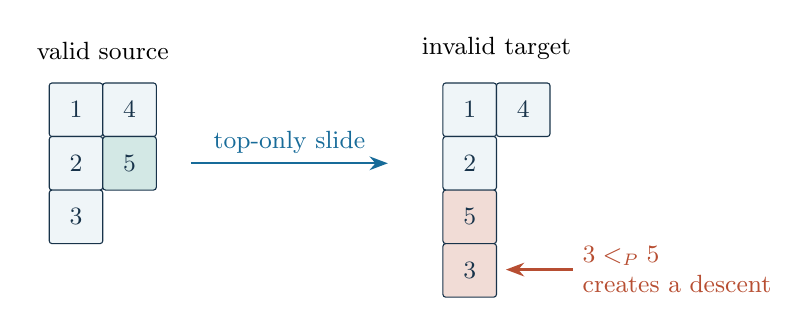
\begin{tikzpicture}[font=\small,>=Stealth]
\begin{scope}
\cell{0}{2.04}{1}{pale}\cell{.68}{2.04}{4}{pale}
\cell{0}{1.36}{2}{pale}\cell{.68}{1.36}{5}{teal!18}
\cell{0}{.68}{3}{pale}
\node[above] at (.68,2.9) {valid source};
\end{scope}
\draw[->,thick,blue] (1.8,1.7)--node[above]{top-only slide}(4.3,1.7);
\begin{scope}[xshift=5cm]
\cell{0}{2.04}{1}{pale}\cell{.68}{2.04}{4}{pale}
\cell{0}{1.36}{2}{pale}\cell{0}{.68}{5}{rust!20}
\cell{0}{0}{3}{rust!20}
\node[above] at (.68,2.9) {invalid target};
\draw[->,rust,thick] (1.65,.35)--(.8,.35);
\node[right,text=rust,align=left] at (1.65,.35) {$3<_P5$\\creates a descent};
\end{scope}
\end{tikzpicture}
\caption{A five-vertex failure with $h=(3,4,4,5,5)$. The graph has edges
$12,13,23,24,34,45$ and is connected. The poset has height two.
The inversion degree is $2$; unchanged weight does not repair invalidity.}
\label{fig:failure}
\end{figure}

There is a stronger obstruction than the failure of one algorithm.

\begin{theorem}[No unrestricted two-sector injection]\label{thm:count}
For every $n\ge5$, in the total order on $[n]$, there are more tableaux of
shape $(2,2,1^{n-4})$ than of shape $(2,1^{n-2})$. No injection from the
entire former set into the latter exists.
\end{theorem}
\begin{proof}
These are standard Young tableaux. Transposing reduces the counts to shapes
$(n-2,2)$ and $(n-1,1)$. For the latter, the sole entry in the second row can
be any of $2,\ldots,n$, giving $n-1$ choices. For the former, choose two
second-row entries from $\{2,\ldots,n\}$; every pair is valid except
$\{2,3\}$. Indeed the top-left entry is $1$, and the next first-row entry
is smaller than the larger chosen entry unless the pair is $\{2,3\}$.
The count is $\binom{n-1}{2}-1=n(n-3)/2$.
At $n=5$ this exceeds $n-1$ by one; the difference increases by $n-2$
when $n$ increases to $n+1$. It is therefore positive for every $n\ge5$.
\end{proof}

At five vertices the missing determinant sectors are visible directly:
\begin{equation}\label{eq:five}
 [e_{4,1}]X_G=F_{2111}-F_{221}-F_{311}+F_{32}+F_{41}-2F_5.
\end{equation}
For a total order every $F_\mu$ is the number of standard tableaux of shape
$\mu$, and the six terms in \eqref{eq:five} are $4-5-6+5+4-2=0$.
The graph is edgeless, so $X_G=e_1^5$. The incomplete two-sector expression
would instead give $-1$. This is a proof obstruction, not a counterexample to
elementary positivity.

\begin{figure}[ht]
\centering
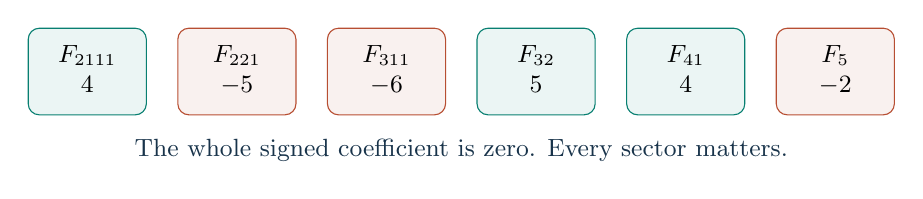
\begin{tikzpicture}[font=\small]
\foreach \x/\lab/\num/\col in {0/2111/4/teal,1.9/221/-5/rust,3.8/311/-6/rust,5.7/32/5/teal,7.6/41/4/teal,9.5/5/-2/rust}{
\node[draw=\col,fill=\col!8,rounded corners,minimum width=1.5cm,minimum height=1.1cm] at (\x,0) {\begin{tabular}{c}$F_{\lab}$\\$\num$\end{tabular}};
}
\node[text=ink] at (4.75,-1) {The whole signed coefficient is zero. Every sector matters.};
\end{tikzpicture}
\caption{The complete dual Jacobi--Trudi cancellation for $e_{4,1}$ in the
five-vertex total order. A wider-shape term cannot be silently dropped.}
\end{figure}

The earlier top-only arm--leg rule also fails its positivity requirement.
For $h=(2,2,3)$, the valid hook with first row $(1,3)$ and leg $(2)$ has
negative sign. The proposed move of $3$ above $2$ is invalid since
$2<_P3$; the reverse move needs $1<_P2$, which is false. It is a negative
fixed point. The established hook involution permits moves at other leg
positions \cite{sagantom}.

\section{The correct insertion and its inverse}

\tagline{Known construction, independently recovered; attribution: Cho--Huh, Section 3.1}
The needed change is to move $b$ farther down when the boundary is blocked.
The construction below is the injection $\psi_\ell$ of Cho--Huh
\cite{chohuh}; it is reproduced, not proposed as a new discovery.

\begin{definition}[Comparable-prefix insertion]
Write the singleton suffix as $C D$, where $C=(c_1,\ldots,c_r)$ is its
longest initial block with $c_i<_P b$ for every $i$. Replace
\[
 \text{front},\ (a,b),\ C,\ D
 \quad\longmapsto\quad
 \text{front},\ (a),\ C,\ (b),\ D.
\]
Call this map $B$. Entries of $C,D$ are singleton rows. The front consists
of the preceding two-cell rows.
\end{definition}

\begin{figure}[ht]
\centering
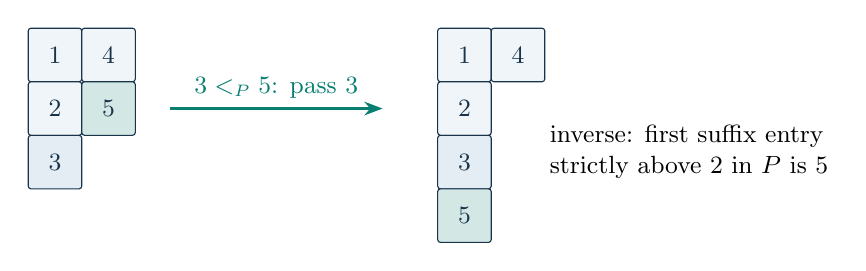
\begin{tikzpicture}[font=\small,>=Stealth]
\begin{scope}
\cell{0}{2.04}{1}{pale}\cell{.68}{2.04}{4}{pale}
\cell{0}{1.36}{2}{pale}\cell{.68}{1.36}{5}{teal!18}
\cell{0}{.68}{3}{blue!12}
\end{scope}
\draw[->,thick,teal] (1.8,1.7)--node[above] {$3<_P5$: pass $3$}(4.5,1.7);
\begin{scope}[xshift=5.2cm]
\cell{0}{2.04}{1}{pale}\cell{.68}{2.04}{4}{pale}
\cell{0}{1.36}{2}{pale}\cell{0}{.68}{3}{blue!12}
\cell{0}{0}{5}{teal!18}
\node[align=left,right] at (1.3,1.15) {inverse: first suffix entry\\strictly above $2$ in $P$ is $5$};
\end{scope}
\end{tikzpicture}
\caption{The repaired map on the same connected example. The exchanged
labels $3,5$ are comparable, so they are not an incomparability edge and no
graph inversion changes.}
\end{figure}

\begin{theorem}[Validity and weight]\label{thm:bubblevalid}
For every finite poset, $B$ sends valid tableaux of shape $(2^{k+1},1^m)$
to valid tableaux of shape $(2^k,1^{m+2})$. It preserves $\inv_G$ for the
incomparability graph.
\end{theorem}
\begin{proof}
After removing $b$, the original first column is unchanged. Insert $b$ after
$C$. The entry immediately above it is either $a$ or the last entry of $C$;
both are smaller than $b$ in $P$. If a following entry exists, it is not
smaller than $b$ by maximality of $C$. The new adjacent column comparisons
are therefore valid. Other comparisons are inherited, and rows are chains.
The filling remains bijective. The row relation of $b$ with $a$ changes from
the same row to a later row, and $b$ passes the entries of $C$. Each such
pair is comparable, hence is not an edge of $G$. All edge orders are unchanged.
\end{proof}

\begin{theorem}[Height-two injection]\label{thm:injection}
If $P$ contains no strict chain of three elements, then $B$ is injective.
Its inverse on its image selects the first singleton entry $x$ below $a$
such that $a<_P x$, removes it, and restores $(a,x)$ as the final two-cell row.
\end{theorem}
\begin{proof}
The moved entry $b$ satisfies $a<_P b$. Every singleton crossed before it
satisfies $c_i<_P b$. If $a<_P c_i$ held, then $a<_P c_i<_P b$ would be a
three-element chain. Thus no earlier singleton is eligible, and $b$ is
exactly the first eligible entry. Extracting it recovers $b$ and the entire
original suffix in order, as well as the unchanged front and $a$. This is a
left inverse, proving injectivity.
\end{proof}

The hypothesis is essential for this inverse. In the five-element total
order, $(12,34,5)$ and $(12,35,4)$ both map to $(12,3,4,5)$.
The map remains valid and weight preserving, but is no longer injective.
Changing insertion depth alone does not solve the unrestricted problem.

\section{A complete mathematical positivity corollary in height two}

Suppose $P_h$ has height at most two. Every tableau row then has length at
most two. Write
\[
 \mu_j=(2^j,1^{n-2j}),\qquad F_j(q)=F_{\mu_j}(q),
 \quad 0\le j\le\lfloor n/2\rfloor,
\]
Outside that range we define $\PT_{\mu_j}(P_h)=\varnothing$ and $F_j=0$,
without assigning a partition to an expression with a negative exponent.
For $1\le j\le\lfloor n/2\rfloor$, the two-column determinant is
\[
 s_{\mu_j}=e_{n-j}e_j-e_{n-j+1}e_{j-1},\qquad s_{\mu_0}=e_n.
\]
Collecting terms in \eqref{eq:schur} gives, for $0\le k\le\lfloor n/2\rfloor$,
\begin{equation}\label{eq:twosectors}
 c_{(n-k,k)}(q)=F_k(q)-F_{k+1}(q),
\end{equation}
where a zero part is omitted. If $n=2k$ the second term is zero.
Coefficients indexed by partitions with more than two parts vanish.

\begin{theorem}[Height-two positivity; Cho--Huh]\label{thm:positive}
For every natural unit interval order $P_h$ of height at most two, all
elementary coefficients of $X_{G_h}(\mathbf x;q)$ belong to $\N[q]$.
More precisely,
\[
 c_{(n-k,k)}(q)=
 \sum_{U\in\PT_{\mu_k}(P_h)\setminus B(\PT_{\mu_{k+1}}(P_h))}
 q^{\inv_{G_h}(U)}.
\]
\end{theorem}
\begin{proof}
For $\mu_{k+1}$ the map $B$ is precisely the valid injection of
Theorems~\ref{thm:bubblevalid}--\ref{thm:injection}, with $k$ two-cell front
rows. It preserves every inversion degree. Subtract its image from the
positive set in \eqref{eq:twosectors}; all remaining monomials have coefficient
$+1$. When the source is empty the assertion is immediate.
\end{proof}

Equivalently, on the disjoint union of a negative copy of the source and a
positive copy of the target, pair each source with its image. Fix the other
positive objects. This is a sign-reversing, weight-preserving involution with
positive fixed points. Both the signed sets and the injection are necessary;
an isolated flag-toggling lemma does not establish their existence.

\section{Lean: what was actually checked}

The project uses Lean 4.34.0 and \texttt{Std}, without a Mathlib download.
Its actual tableau predicate requires a distinct vertex list, a permutation
of that list as the flattened filling, nonempty chain rows, a partition
shape, and every adjacent column condition. This prevents the semantic gap
in the earlier boundary object, which omitted the comparison below the moved
entry.

\subsection{Complete families and degreewise cancellation}

Let $\mathcal T_k=\PT_{(2^k,1^{n-2k})}(P)$ when $2k\le n$, and let
$\mathcal T_k=\varnothing$ otherwise. Put
$\mathcal S_k=\mathcal T_k\setminus B_k(\mathcal T_{k+1})$, where $B_k$
is insertion at the final two-cell row. For a finite family $A$, write
$C_d(A)=\#\{T\in A:\inv_G(T)=d\}$.

\begin{theorem}[Formal degreewise survivor identity]\label{thm:formalcounts}
For every finite poset of height at most two and every $k,d\in\N$,
\[
 C_d(\mathcal T_k)=C_d(\mathcal T_{k+1})+C_d(\mathcal S_k).
\]
The empty vertex set has one empty tableau of degree zero. A single vertex
also has one tableau of degree zero. At either an odd or even maximal index,
the next source is empty and every target is a survivor.
\end{theorem}
\begin{proof}
Generate every filling of the specified shape from the finite vertex list,
retain exactly the actual tableaux, and remove duplicates. Membership in this
family is proved equivalent to tableau validity and the exact row-length list;
completeness is not an input assumption. The source shape determines the split
index $k$. Theorem~\ref{thm:injection} gives a weight-preserving injection into
the target family. Its image in degree $d$ has exactly
$C_d(\mathcal T_{k+1})$ objects. Partitioning the target into this image and its
complement proves the equality using addition of natural counts. The guard
$2k\le n$ handles every out-of-range index before forming $n-2k$.
\end{proof}

\begin{figure}[ht]
\centering
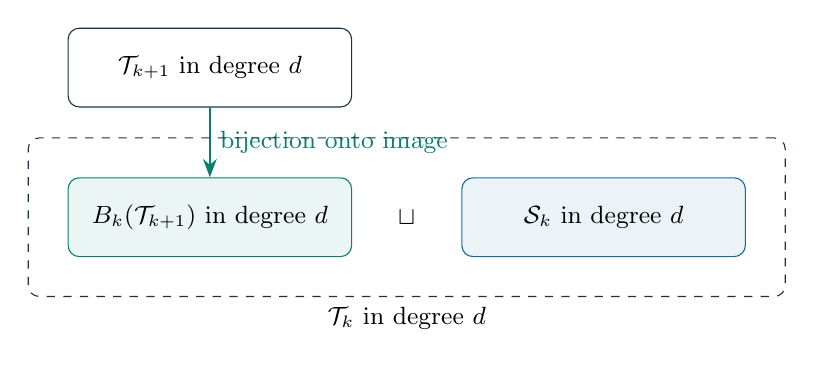
\begin{tikzpicture}[font=\small,>=Stealth]
\node[draw=ink,rounded corners,minimum width=3.6cm,minimum height=1cm]
 (source) at (0,0) {$\mathcal T_{k+1}$ in degree $d$};
\node[draw=teal,fill=teal!8,rounded corners,minimum width=3.6cm,minimum height=1cm]
 (image) at (0,-1.9) {$B_k(\mathcal T_{k+1})$ in degree $d$};
\node[draw=blue,fill=blue!8,rounded corners,minimum width=3.6cm,minimum height=1cm]
 (survivor) at (5,-1.9) {$\mathcal S_k$ in degree $d$};
\draw[->,thick,teal] (source)--node[right]{bijection onto image}(image);
\node at (2.5,-1.9) {$\sqcup$};
\node[draw=ink,dashed,rounded corners,fit=(image)(survivor),inner sep=5mm,
 label=below:{$\mathcal T_k$ in degree $d$}] {};
\end{tikzpicture}
\caption{The checked finite decomposition. The weight-preserving injection
identifies the source with one part of the target; the other part consists
of survivors. No subtraction or polynomial-coefficient assumption is used.}
\end{figure}

The declarations \texttt{mem\_family} and \texttt{family\_nodup} establish the
enumeration properties. The all-index result is
\texttt{height\_two\_degreewise\_cancellation}. For a relation defined only
on the vertex set, \texttt{finiteRelation} extends it by false outside that
set, and \texttt{finite\_height\_two\_degreewise\_cancellation} requires
asymmetry and height only on those vertices. The following table records the
remaining assurance boundary.

\begin{center}
\small
\begin{tabular}{p{.39\linewidth}p{.51\linewidth}}
\toprule
Mathematical obligation & Verification boundary\\
\midrule
Exact top-only slide criterion & General actual-tableau theorem
\texttt{demote\_valid\_iff}\\[2mm]
Unchanged word for the top-only slide & General equality
\texttt{flatten\_before\_after}\\[2mm]
Five-vertex invalidity & Explicit source validity and target invalidity\\[2mm]
Comparable-prefix insertion & Recursive insertion and first-eligible extraction,
with a general left inverse; actual-tableau validity and injectivity\\[2mm]
Tableau inversion weight & The row-to-word correspondence and the actual
tableau weight-preservation theorem are checked in Lean\\[2mm]
Complete fixed-shape families & Exact membership, no duplicates, derived
split index, and the family-level injection are checked\\[2mm]
Survivor counts & Theorem~\ref{thm:formalcounts}, for all indices and degrees,
including empty and singleton boundaries, is checked\\[2mm]
Symmetric-function bridge & The imported Schur expansion, determinant
coefficient identity, and final elementary positivity corollary are written
arguments; they are not formalized in Lean\\
\bottomrule
\end{tabular}
\end{center}

The accompanying Lean README identifies every checked declaration, its
assumptions, and its axiom dependencies. A successful build establishes those
formal statements relative to Lean's kernel and listed standard axioms. It
does not certify the informal translation or the general positivity problem.
The source contains no proof placeholders or new axioms. A separate semantic
review found no defect in these finite-family statements. The recorded
reproduction builds all three modules in a fresh temporary directory and
checks their sources directly; all 31 printed dependency lists use only
\texttt{propext}, \texttt{Quot.sound}, and \texttt{Classical.choice}.

The remaining height-two formalization gap is the equality between the actual
proper-coloring polynomial and the elementary expansion. Theorem~\ref{thm:formalcounts}
does not supply the Schur expansion or the basis change in
\eqref{eq:schur}--\eqref{eq:djt}. Those identities still require their own
formal development or a verified, correctly attributed import.

\section{Finite evidence from two independent calculations}

The primary enumerator generates permutations of labels, filters by actual
tableau conditions, computes inversion degrees, and expands the integer
determinant \eqref{eq:djt}. A separate oracle enumerates proper colorings
with prescribed ordered color multiplicities and expands elementary products
as choices of subsets. Exact rational elimination recovers elementary
coefficients. The oracle uses neither tableaux nor Jacobi--Trudi.

The two methods agree for every Hessenberg vector through five vertices.
The comparable-prefix map is additionally tested on all height-two vectors
through seven vertices. These are finite checks of implementations, not
inductive proofs. The deterministic verification script and JSON reports
record the exact ranges and counts.

\begin{center}
\small
\begin{tabular}{lrrrrrr}
\toprule
Number of vertices & 2 & 3 & 4 & 5 & 6 & 7\\
\midrule
Height-two orders & 2 & 4 & 8 & 16 & 32 & 64\\
Source tableaux checked & 1 & 5 & 36 & 282 & 2730 & 30420\\
Failures & 0 & 0 & 0 & 0 & 0 & 0\\
\bottomrule
\end{tabular}
\end{center}

For the connected five-vertex witness from Figure~\ref{fig:failure}, both
methods give
\begin{align*}
 c_5(q)&=1+3q+4q^2+4q^3+4q^4+3q^5+q^6,\\
 c_{4,1}(q)&=q+3q^2+4q^3+3q^4+q^5,\\
 c_{3,2}(q)&=q^2+2q^3+q^4,
\end{align*}
and no other nonzero coefficients. The false top-only slide and the true
positivity statement can therefore be tested on the same small object.

The checks count graph inversions exactly, not a surrogate statistic. They
also test the empty graph, complete graphs, the four-vertex path, the missing
suffix boundary, and collisions when the height hypothesis is removed.
The largest test range is deliberately explicit; no claim about larger
instances follows from the enumeration alone.

\section{What the general solution still needs}

The repaired map closes the height-two argument, a known result. For general
natural unit interval orders, rows can be longer. The full determinant then
has additional signed sectors, and the shape-to-shape strategy is impossible
in the form proposed in the earlier notes (Theorem~\ref{thm:count}).
A proof using this route would need all of the following:
\begin{enumerate}
\item An actual configuration space of tableaux paired with determinant
permutations, including zero-index factors and every contributing shape.
\item A uniform map preserving validity and inversion degree while allowing
movement between the wider signed sectors.
\item An explicit inverse or a terminating cancellation argument, with a
proof of positive fixed points and no unpaired negative configurations.
\item A formal bridge from those configurations to the exact elementary
coefficients. A finite lookup table cannot replace it.
\end{enumerate}
The $n=5$ total-order identity \eqref{eq:five} is a minimal regression test
for a candidate generalization. The connected height-two witness tests the
local boundary separately. A future proposed map must pass both before its
general proof is credible.

This investigation does not establish a new open-problem solution. It
replaces an invalid purported solution with precise obstructions, a complete
restricted mathematical proof, and a formally checked combinatorial core.
No inference about AI architecture quality follows from this research run.

\begin{thebibliography}{9}
\bibitem{chohuh} S. Cho and J. Huh.
\emph{On $e$-positivity and $e$-unimodality of chromatic quasisymmetric functions}.
SIAM J. Discrete Math. 33 (2019), 2286--2315.
Section 3.1, injection $\psi_\ell$ and Theorem 3.3.
\href{https://arxiv.org/abs/1711.07152}{arXiv:1711.07152}.
\bibitem{sw} J. Shareshian and M. L. Wachs.
\emph{Chromatic quasisymmetric functions}.
Adv. Math. 295 (2016), 497--551. Definition 6.1 and Theorem 6.3.
\href{https://arxiv.org/abs/1405.4629}{arXiv:1405.4629}.
\bibitem{hikita} T. Hikita.
\emph{A proof of the Stanley--Stembridge conjecture}.
Version 2, 25 December 2025.
\href{https://arxiv.org/abs/2410.12758}{arXiv:2410.12758}.
\bibitem{sagantom} B. E. Sagan and F. Tom.
\emph{Chromatic symmetric functions and change of basis}.
Algebraic Combinatorics (2026).
\href{https://doi.org/10.5802/alco.468}{doi:10.5802/alco.468}.
\bibitem{openai} OpenAI.
\emph{Elementary positivity of chromatic quasisymmetric functions}.
Preprint, 24 September 2026, Theorem 1.1.
\href{https://github.com/openai/math/blob/main/preprints/Elementary-Positivity-of-Chromatic-Quasisymmetric-Functions-September-24-2026/paper.pdf}{Primary preprint}.
Statement and selected proof sections inspected; full proof unverified here.
\end{thebibliography}
\end{document}
